\documentclass{minimal}
\usepackage{epsfig,color}
\usepackage[papersize={576.00bp,432.00bp},text={576.00bp,432.00bp}]{geometry}
\begin{document}
\centering
% Title: glps_renderer figure
% Creator: GL2PS 1.3.8, (C) 1999-2012 C. Geuzaine
% For: Octave
% CreationDate: Sun Jul 19 17:12:05 2015
\setlength{\unitlength}{1pt}
\begin{picture}(0,0)
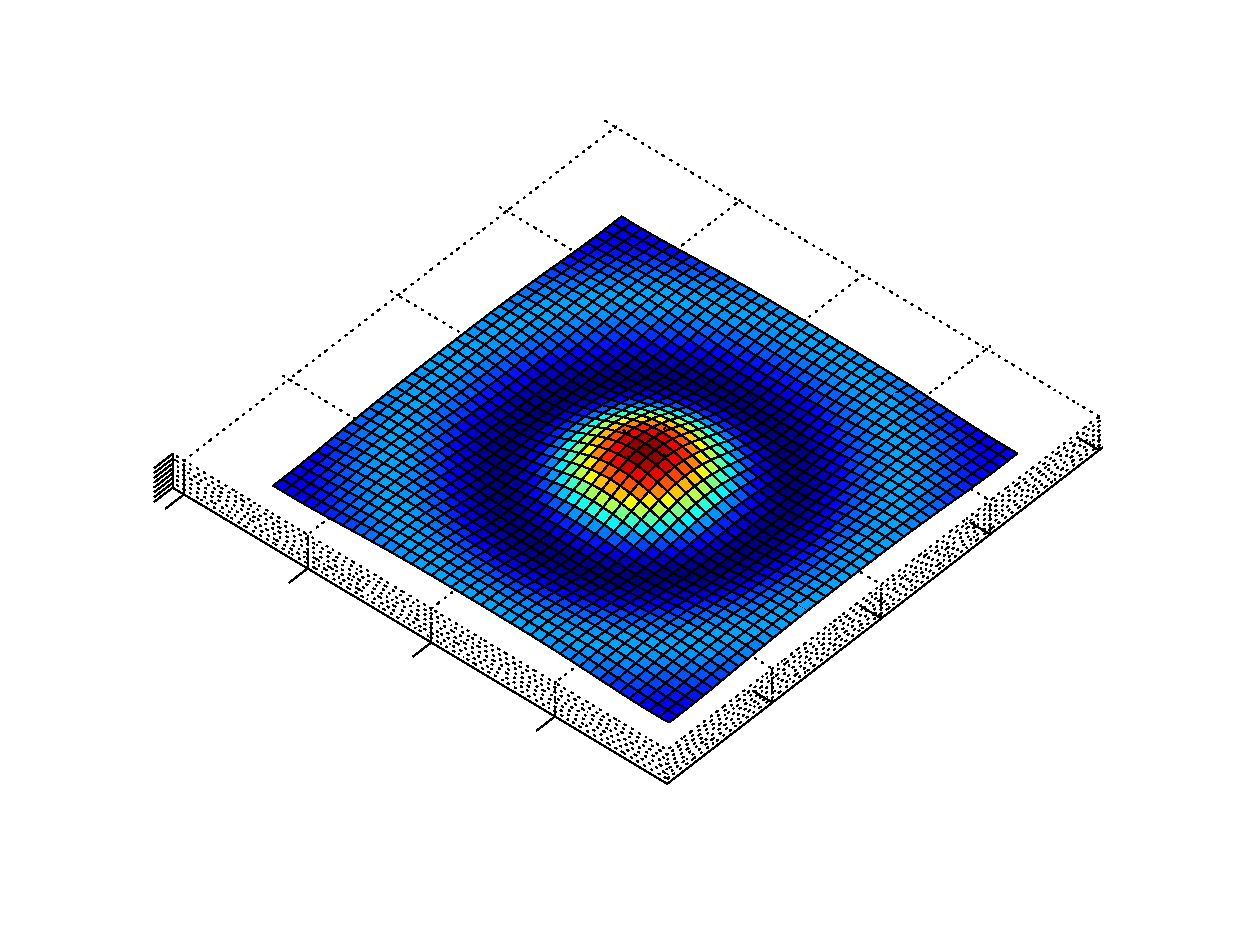
\includegraphics{test_epslatex-inc}
\end{picture}%
\begin{picture}(576,432)(0,0)
\fontsize{10}{0}
\selectfont\put(376.652,94.3171){\makebox(0,0)[tl]{\textcolor[rgb]{0,0,0}{{5}}}}
\fontsize{10}{0}
\selectfont\put(428.9,134.687){\makebox(0,0)[tl]{\textcolor[rgb]{0,0,0}{{0}}}}
\fontsize{10}{0}
\selectfont\put(481.147,175.057){\makebox(0,0)[tl]{\textcolor[rgb]{0,0,0}{{-5}}}}
\fontsize{10}{0}
\selectfont\put(533.395,215.427){\makebox(0,0)[tl]{\textcolor[rgb]{0,0,0}{{-10}}}}
\fontsize{10}{0}
\selectfont\put(298.08,393.49){\makebox(0,0)[b]{\textcolor[rgb]{0,0,0}{{Plot the familiar 3-D sombrero function:$z = \frac{\sin\left(\sqrt{x^2 + y^2}\right)}{\sqrt{x^2 + y^2}}$}}}}
\fontsize{10}{0}
\selectfont\put(186.195,121.574){\makebox(0,0)[tr]{\textcolor[rgb]{0,0,0}{{0}}}}
\fontsize{10}{0}
\selectfont\put(245.548,86.0364){\makebox(0,0)[tr]{\textcolor[rgb]{0,0,0}{{5}}}}
\fontsize{10}{0}
\selectfont\put(126.843,157.111){\makebox(0,0)[tr]{\textcolor[rgb]{0,0,0}{{-5}}}}
\fontsize{10}{0}
\selectfont\put(67.4901,192.648){\makebox(0,0)[tr]{\textcolor[rgb]{0,0,0}{{-10}}}}
\fontsize{10}{0}
\selectfont\put(62.0787,195.888){\makebox(0,0)[tr]{\textcolor[rgb]{0,0,0}{{-0.4}}}}
\fontsize{10}{0}
\selectfont\put(62.0787,198.207){\makebox(0,0)[tr]{\textcolor[rgb]{0,0,0}{{-0.2}}}}
\fontsize{10}{0}
\selectfont\put(62.0787,200.526){\makebox(0,0)[tr]{\textcolor[rgb]{0,0,0}{{0}}}}
\fontsize{10}{0}
\selectfont\put(62.0787,202.844){\makebox(0,0)[tr]{\textcolor[rgb]{0,0,0}{{0.2}}}}
\fontsize{10}{0}
\selectfont\put(62.0787,205.163){\makebox(0,0)[tr]{\textcolor[rgb]{0,0,0}{{0.4}}}}
\fontsize{10}{0}
\selectfont\put(62.0787,207.481){\makebox(0,0)[tr]{\textcolor[rgb]{0,0,0}{{0.6}}}}
\fontsize{10}{0}
\selectfont\put(62.0787,209.8){\makebox(0,0)[tr]{\textcolor[rgb]{0,0,0}{{0.8}}}}
\fontsize{10}{0}
\selectfont\put(62.0787,212.118){\makebox(0,0)[tr]{\textcolor[rgb]{0,0,0}{{1}}}}
\end{picture}
\end{document}
